\chapter{ActivityNet系统设计}

\section{SAE概述}
考虑到系统将来的可扩展性,我们选择SAE作为系统底层架构。SAE全称为Social Analytic Engine,即社交网络分析引擎,是清华大学计算机系KEG研究组开发的一套社交网络分析平台。可以提供以下功能:
\begin{enumerate}
\item 存储和快速检索极大规模社交网络的数据
\item 提供最新的社交网络分析算法和机器学习算法,如话题模型(Topic Model), 影响力最大化(Influence Maximization)等
\item 提供通用的网络分析引擎和机器学习引擎.
\end{enumerate}

\begin{figure}[!h]
\centering
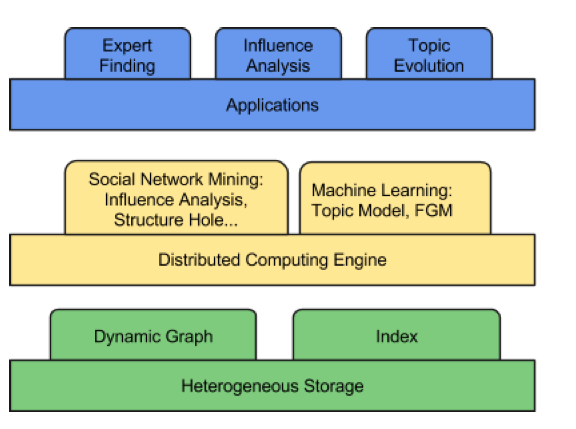
\includegraphics[width=0.7\textwidth]{sae.png}
\caption{SAE基本结构}
\label{fig:sae_arch}
\end{figure}

\section{设计目标}
通过ActivityNet,希望实现以下目标:
\begin{itemize}
\item 高效的活动检索
\end{itemize}

\section{底层存储}

\section{界面和功能设计}
ActivityNet以Web站点的形式提供服务。基于成熟的前端框架$Twitter Bootstrap$,简化了开发工作。

\subsection{首页设计}
ActivityNet的首页如图\ref{fig:frontpage}。

\begin{figure}[h]
\centering
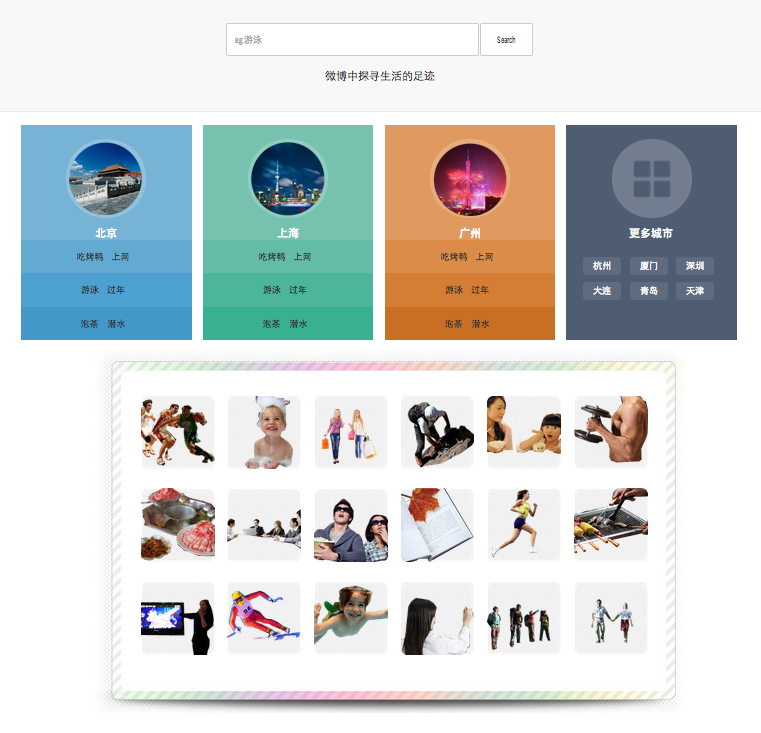
\includegraphics[width=\textwidth]{frontpage.png}
\caption{Activity首页设计}
\label{fig:frontpage}
\end{figure}

首页上我们提供以下功能
\begin{enumerate}
\item 活动搜索框。用户可以自行输入自己希望查询的活动
\item 城市热门活动推荐。我们计算出北京、上海、广州的热门活动,在首页进行推荐。
\item 全网热门活动。基于活动实例抽取结果,我们选择了18个最热门的活动,在首页底部呈现。活动对应的图片是以活动本身为关键词构建GET请求,在百度图片搜索抓取第一张图。自动抓取的个别活动图片不很理想。我们在自动抓取图片后,人工进行一些调整。
\end{enumerate}

\section{二级页面}
用户输入一个查询后,可以进入此活动查询结果的二级页面。例如,输入``烤鸭'',查询结果如图\ref{fig:query_kaoya}

\begin{figure}[h]
\centering
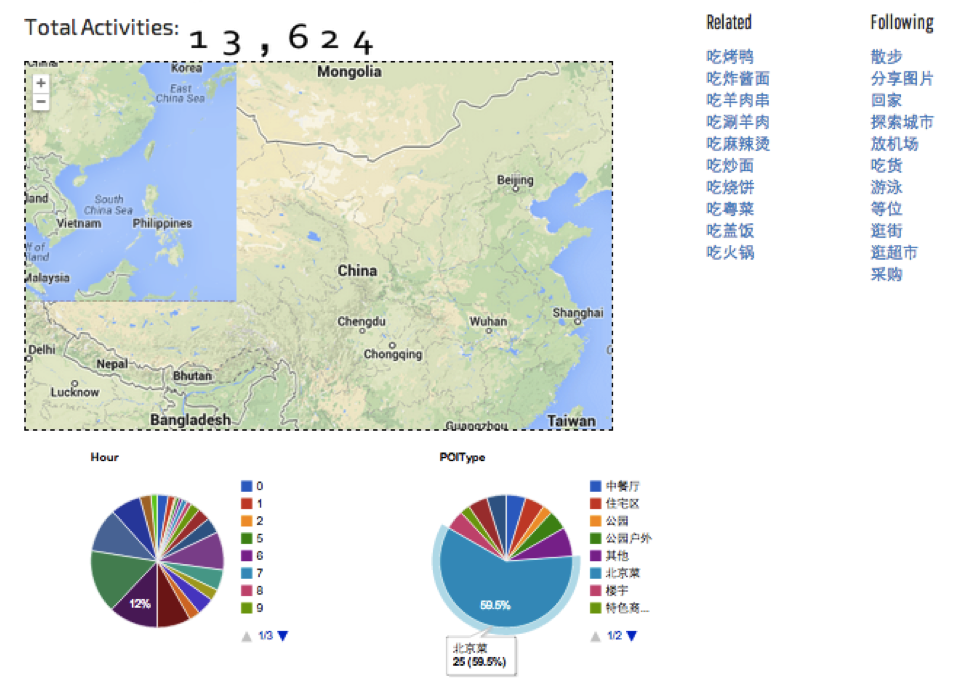
\includegraphics[width=\textwidth]{kaoya.png}
\caption{查询结果}
\label{fig:query_kaoya}
\end{figure}

在左侧,ActivityNet使用Google Map API进行地理信息的可视化。在右侧,首先,我们列出了和查询相关的前10个活动,以相关性排序;其次,利用序列关系抽取的结果,我们列出了此活动经常发生的后续活动。烤鸭是北京的特色菜品,``相关活动''中,我们列出的``炸酱面'',``涮羊肉'',``麻辣烫''也都是北京的特色菜。在序列关系中,ActivityNet提供了``散步'',``回家'',``游泳'',``探索城市'',``逛街'',``逛超市''等活动,是比较合理的。由于概念的抽取无法做到完全的精准,ActivityNet的结果中有一些噪声,为此,我们提供用户反馈机制。如果用户发现返回的结果不是活动,鼠标移上之后会呈现$\times$按钮,点击后会向系统报告错误。

\section{本章小结}
本章从底层架构到界面设计介绍了基于活动信息挖掘的可视化系统ActivityNet。ActivityNet基于SAE(Social Analytic Engined)实现了高效的存储和检索功能,并利用gchart和Google Map API实现信息可视化,有着较好的用户体验。

